\documentclass[]{article}

\usepackage[margin=1.0in]{geometry}
\usepackage{amsmath}
\usepackage{amsfonts}
\usepackage{amsthm}
\usepackage{graphicx}
\usepackage{amssymb}

\usepackage{mathtools}

%opening
\title{Old Attempt Computing the Hausdorff Dimension for Symmetric Schottky Groups}
\author{Alex Karlovitz}
\date{}

\begin{document}
	
	\maketitle

This is work from before I realized the rotational symmetry of the Schottky groups makes Hejhal's algorithm the algorithm break.
I am still saving everything in case I need to look back at it later...

\section*{Mapping to the Upper Half Plane}

Recall that we can map from the upper half plane model to the disk model via the \textit{Cayley transform}
$$
C(z) = \frac{z - i}{z + i}
$$
We can go the other direction by taking the inverse
$$
C^{-1}(w) = i\cdot\frac{1 + w}{1 - w}
$$
Also recall that $C$ and $C^{-1}$ send geodesics to geodesics.

Next, note that we are choosing to center one of our circles of reflection about $1$.
Since $C^{-1}(1) = \infty$, this has the effect of forcing our fundamental domain to be bounded inside $C^{-1}$ of that circle.
See Figure \ref{UHP_FD} for an example.

\begin{figure}[h]
	\centering
	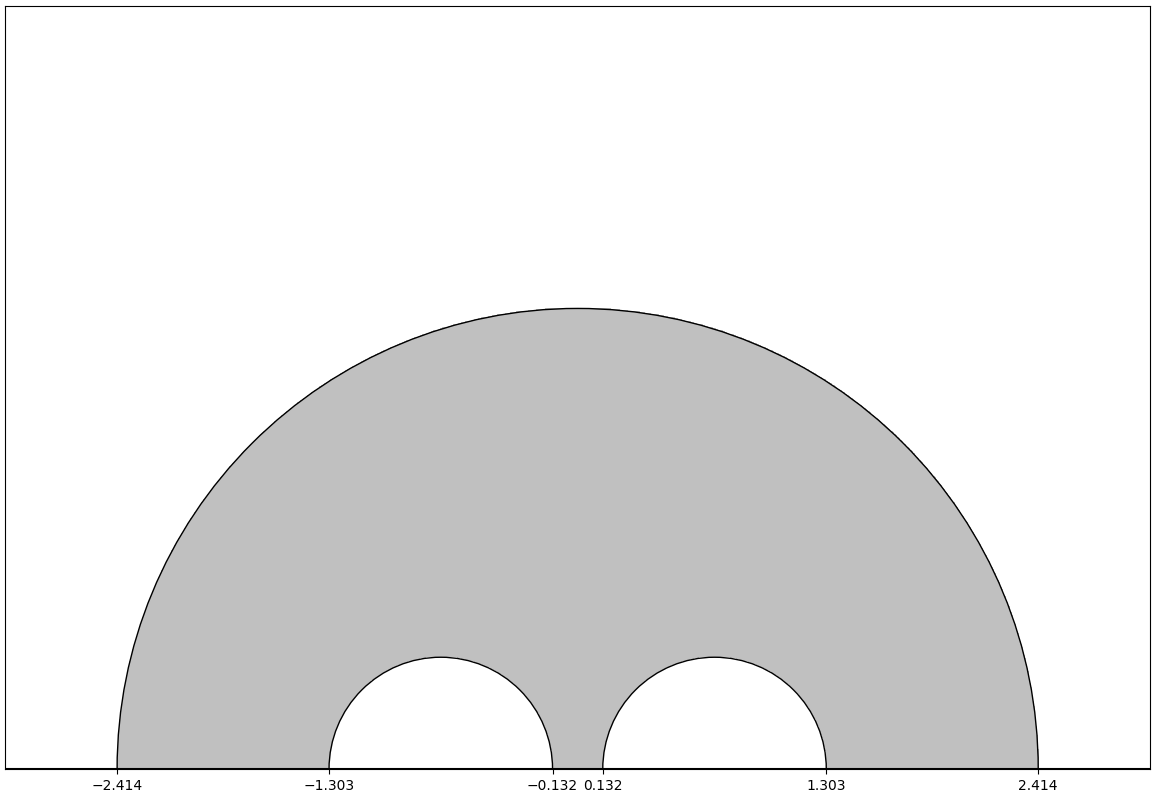
\includegraphics[width=0.6\linewidth]{../UHP_FD.png}
	\caption{The example from Figure \ref{disk_FD} mapped to the upper half plane.}
	\label{UHP_FD}
\end{figure}

\textbf{Note:} this image seems to single out the middle flare as different from the other two, but this is just an artifact of our choice of Cayley transform.
We could just as easily have mapped $e^{\pi i/3}$ or $e^{-\pi i/3}$ to $-1$ instead.
\\

Finally, let's give a name to each of the circles involved.
In the disk, we will call the rightmost circle (which contains the point $1$) $R_1$.
We then proceed counterclockwise and name the next two circles $R_2$ and $R_3$.
The resulting labels in the upper half plane are shown in Figure \ref{UHP_labeled}.

\begin{figure}[h]
	\centering
	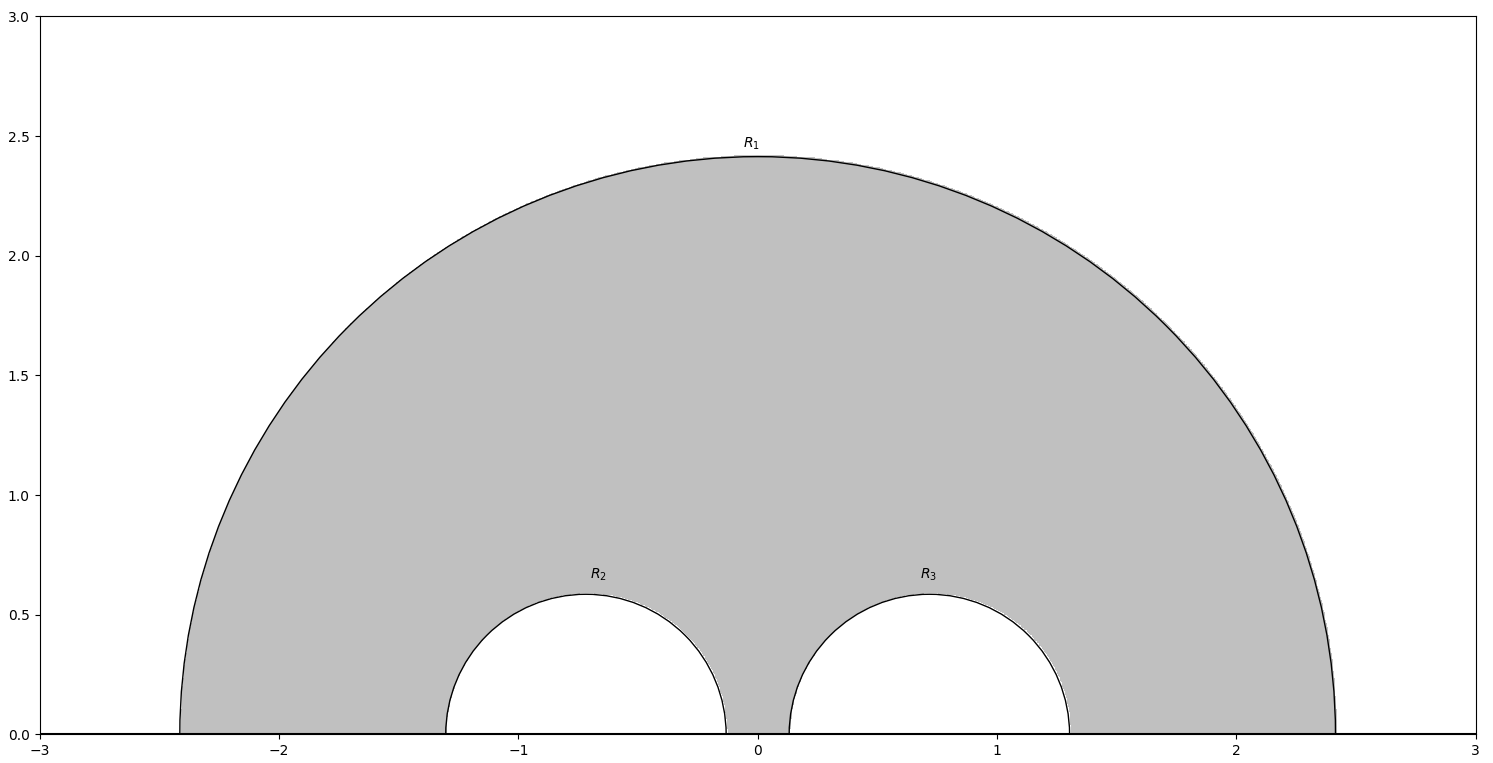
\includegraphics[width=0.6\linewidth]{../UHP_labeled.png}
	\caption{Labeling of the circles from Figure \ref{UHP_FD}.}
	\label{UHP_labeled}
\end{figure}

\subsection*{Identifying Flare Domains}

Let us call the group generated by our three reflections
$$
\Gamma = \langle R_1, R_2, R_3 \rangle
$$
To get a flare domain, we need to identify a hyperbolic element in $\Gamma$ whose axis\footnote{Recall that the \textit{axis} of a hyperbolic matrix is the geodesic whose endpoints are the fixed points of the matrix.} ``cuts off'' a flare in our fundamental domain.
To do this, we first recall that even length words in circle reflections give M\"obius transformations.
Thus, we could look for appropriate hyperbolic matrices by checking small words of even length in our generators.
Indeed, one quickly finds that $R_1R_2, R_1R_3$, and $R_2R_3$ are hyperbolic matrices with appropriate axes (see Figure \ref{UHP_flares}).

\begin{figure}[h]
	\centering
	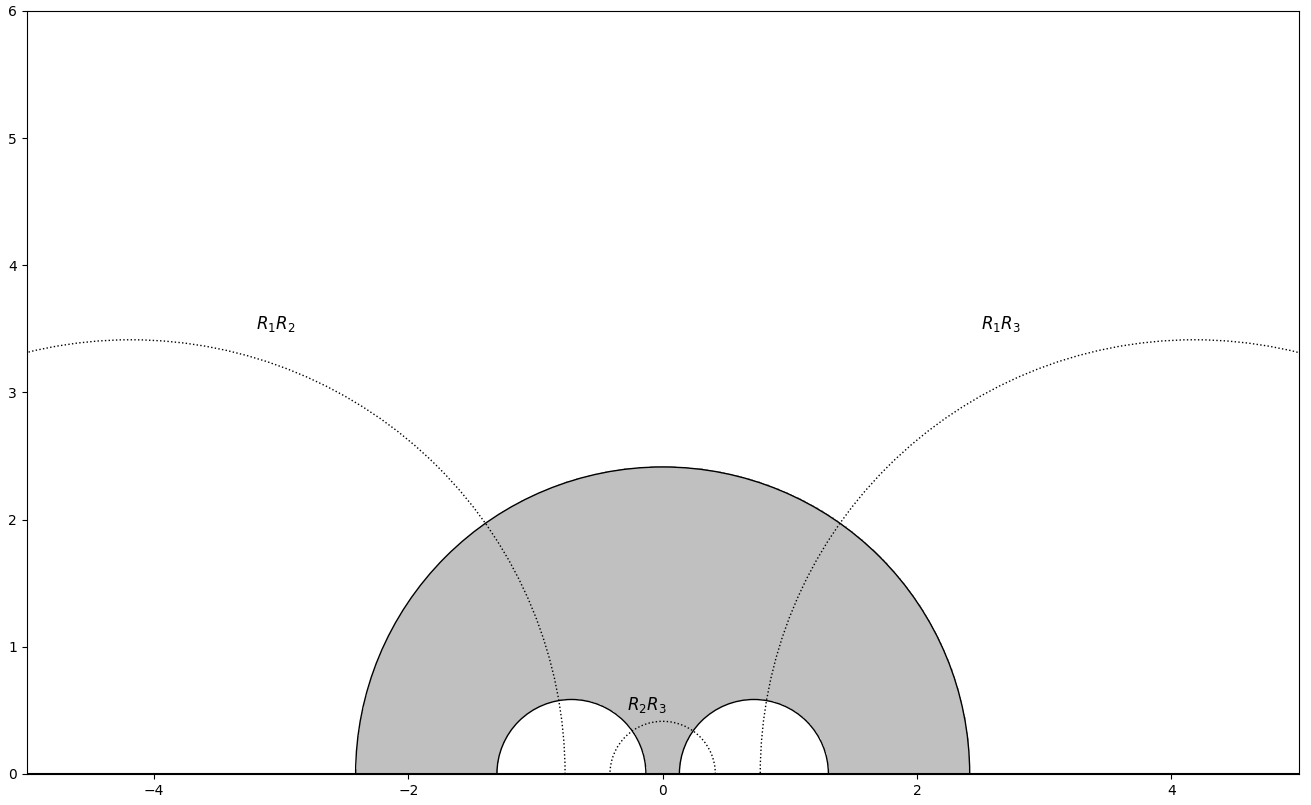
\includegraphics[width=0.6\linewidth]{../UHP_flares.png}
	\caption{Axes cutting off flares labeled with the associated hyperbolic matrices.}
	\label{UHP_flares}
\end{figure}

Let's be a bit more formal in our discussion of flares.
To identify a flare between geodesics $C_1$ and $C_2$, one may look for a geodesic with the following properties:
\begin{itemize}
	\item one endpoint of the geodesic is on the other side of $C_1$ from the flare
	\item the other endpoint is on the other side of $C_2$ from the flare
	\item the geodesic meets $C_1$ and $C_2$ at right angles
\end{itemize}
In our situation, it is always possible to find a hyperbolic element in $\Gamma$ whose axis satisfies these properties.
To see this, one looks in inversive coordinates (see Kontorovich's letter to Bill Duke).
Letting $v_1$ and $v_2$ denote the inversive coordinates for $C_1$ and $C_2$, respectively, one looks for the inversive coordinates $v$ such that
$$
v_1^tQv = 0 ~~~~~ v_2^tQv = 0 ~~~~~ v^tQv = -1
$$
where $Q$ is the quadratic form defining inversive coordinates.
The first two equations give the orthogonality, and the third gives a true vector of inversive coordinates.
Finally, these coordinates give the endpoints of our geodesic.
To find the corresponding M\"obius transformation in $\Gamma$, one searches over all transformations with this axis for the one taking the intersection point with $C_1$ to that of $C_2$.

\clearpage

\section*{Mapping to a Flare Domain}

Let us look at a generic flare: two geodesics separated by positive length interval on the real line, plus a geodesic cutting through both of these at a right angle.
Let the two points on this last geodesic be labeled $z_1 < z_2$, and call the rightmost point of the first geodesic $t$.
See Figure \ref{pre_flare}.
\begin{figure}[h]
	\centering
	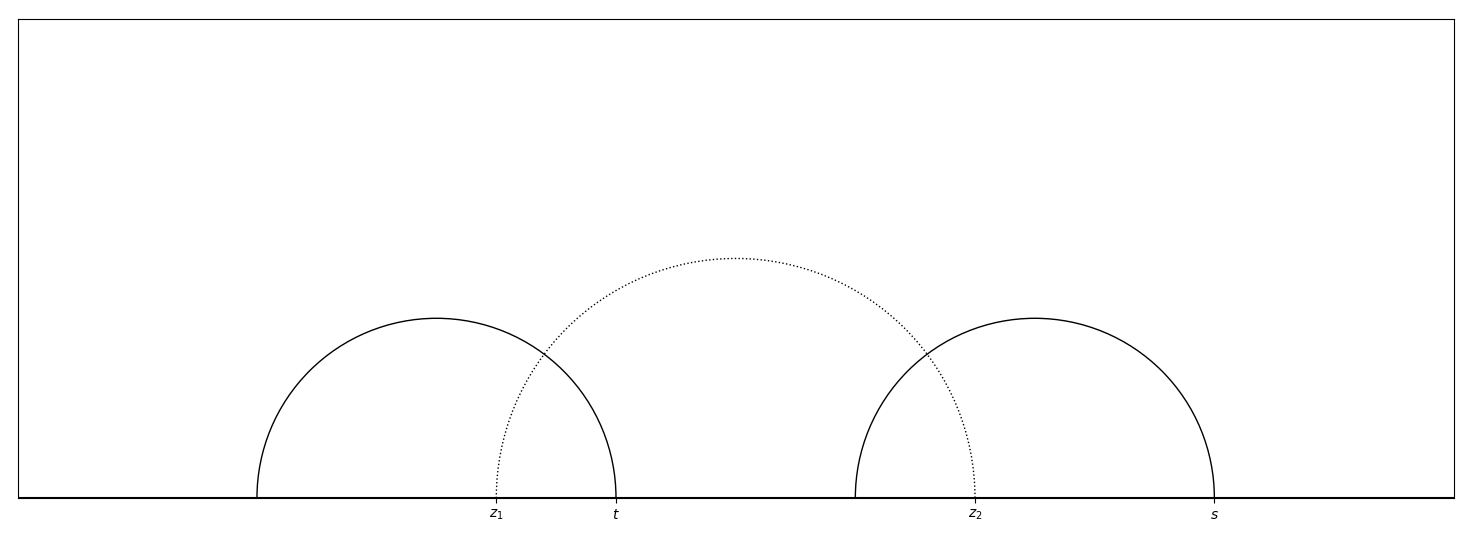
\includegraphics[width=0.6\linewidth]{../labeled_pre_flare.png}
	\caption{A generic flare.}
	\label{pre_flare}
\end{figure}
Now consider the M\"obius transformation
$$
U(z) = \left( \frac{t - z_2}{t - z_1} \right) \frac{z - z_1}{z - z_2}
$$
This function is chosen so that
$$
U(z_1) = 0 ~~~~~ U(z_2) = \infty ~~~~~ U(t) = 1
$$
Thus, applying such a $U$ to a generic flare gives us a \textit{flare domain}.
See Figure \ref{post_flare} for an example.
\begin{figure}[h]
	\centering
	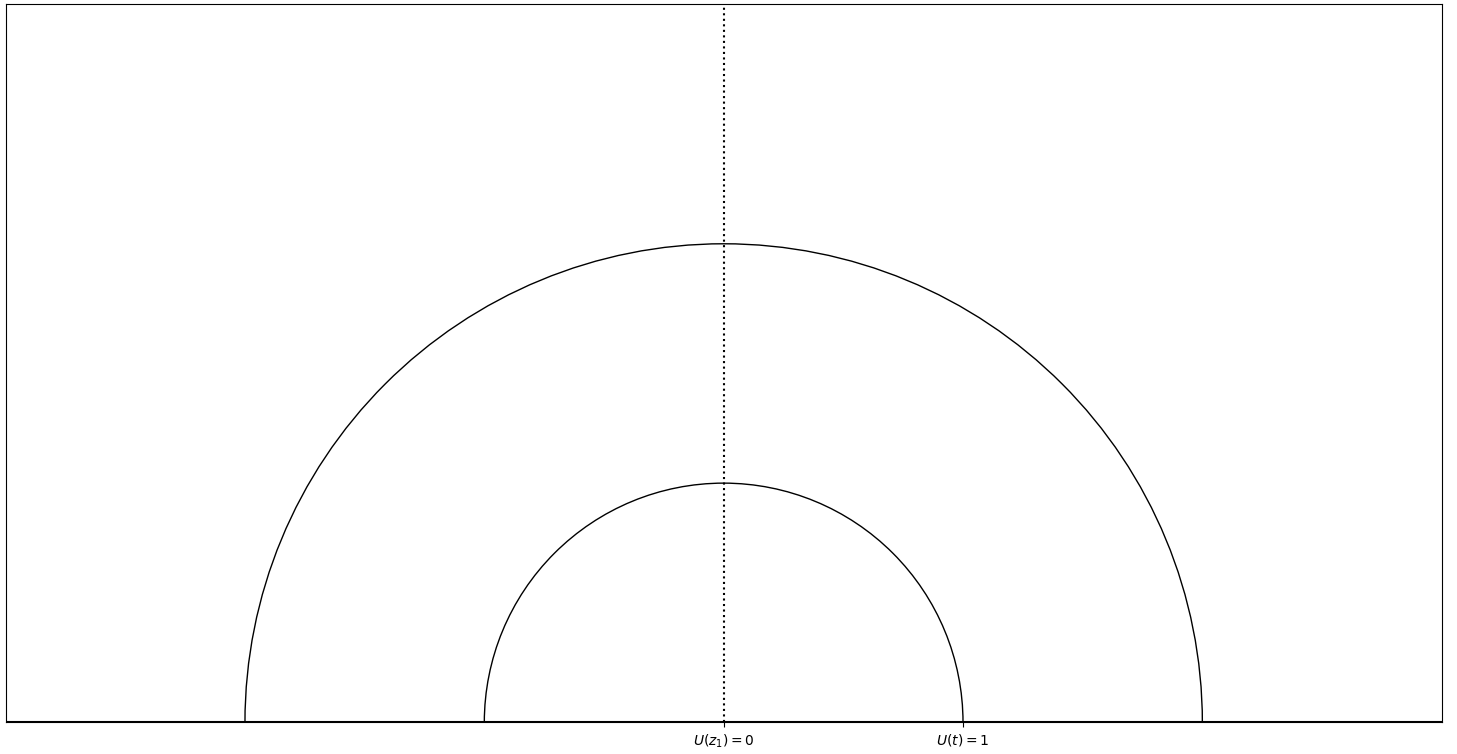
\includegraphics[width=0.6\linewidth]{../labeled_flare.png}
	\caption{A flare domain.}
	\label{post_flare}
\end{figure}

Let's consider our symmetric Schottky group example.
Using the flare cut off by the axis of $R_2R_3$, we get the flare domain pictured in Figure \ref{flare}.
\begin{figure}[h]
	\centering
	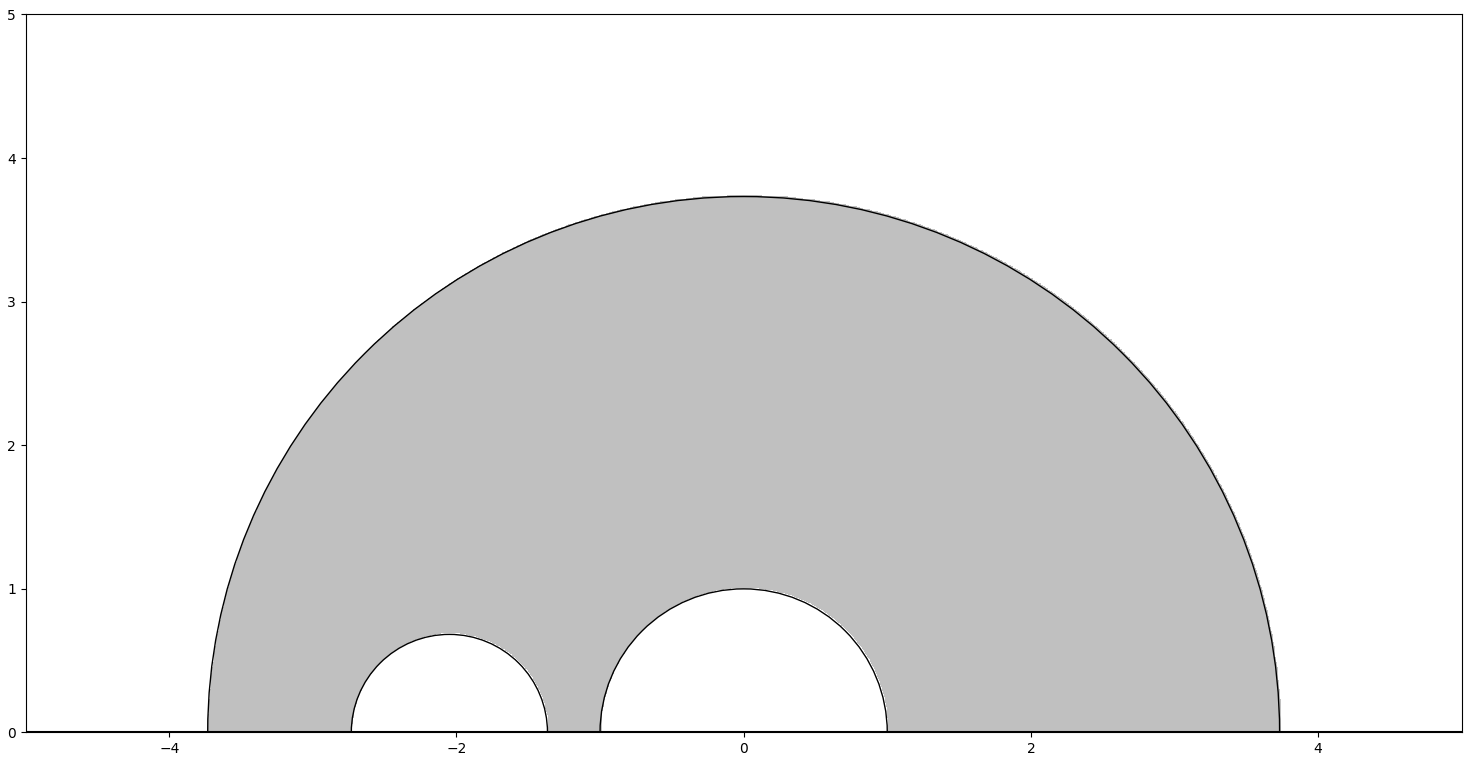
\includegraphics[width=0.6\linewidth]{../flare.png}
	\caption{The flare domain obtained from middle flare in Figure \ref{UHP_flares}.}
	\label{flare}
\end{figure}

\clearpage

\section*{Appendix: Considerations for Choosing Test Points}

Let's consider the action of $R_2R_3$ in the flare domain.
Note that the main purpose of mapping to the flare domain is to convert this hyperbolic transformation into a scaling matrix (of course this is still a hyperbolic transformation, just a very specific and simple one).
Specifically, the action is converted to one of the form
$$
z \mapsto \kappa z
$$
for some $\kappa > 1$.
Furthermore, recall that it is this action which leads to a logarithmic Fourier expansion of Maass forms.
Specifically, if $\phi$ is a Maass form for such a Schottky group, where $\phi(r, \theta)$ is a function of the polar coordinates $(r, \theta)$ in the flare, then
$$
\phi(r, \theta) = \sum_{n\in\mathbb{Z}}g_n(\theta)e\left( n\frac{\log r}{\log \kappa} \right)
$$
But note that $\phi(r, \theta)$ is then automatically invariant under the map $z \mapsto \kappa z$.
So if we take a test point with pullback equal to $\kappa^nz$ for some $n \in \mathbb{Z}, n \neq 0$, we gain \textit{no new information} from equating $\phi$ at this point and its pullback.
\\

Next, recall that our Maass form is also invariant \textit{in the disk model} under rotation by $2\pi/3$.
Let's draw the $2\pi/3$-sector containing our flare after mapping over to the flare domain.
This is shown in Figure \ref{flare_with_sector}.
\begin{figure}[h]
	\centering
	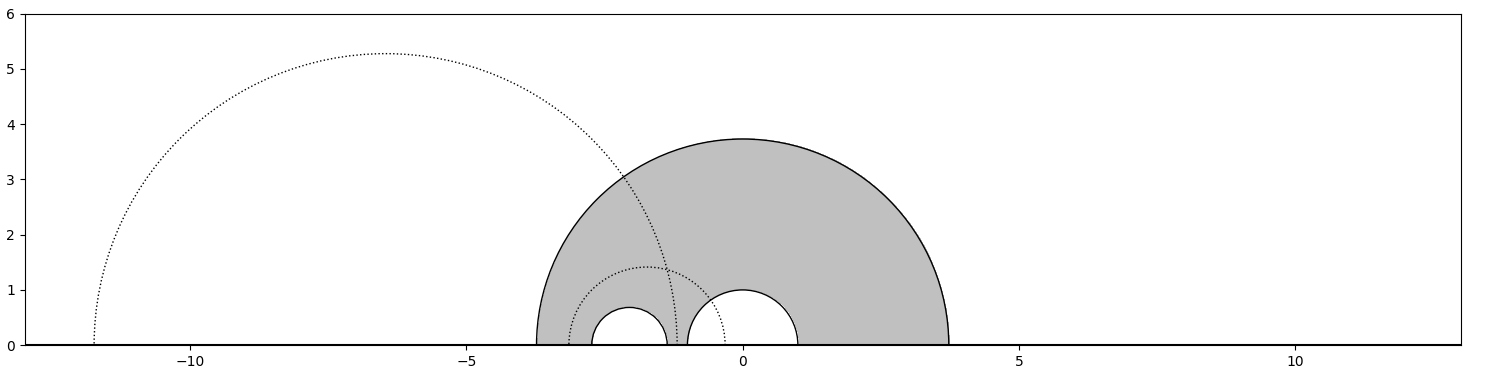
\includegraphics[width=\linewidth]{../flare_with_sector.png}
	\caption{The $2\pi/3$-sector containing our flare.}
	\label{flare_with_sector}
\end{figure}
As we have argued, the only viable test points are those which are inside our chosen sector and whose pullback is not just multiplication by a power of $\kappa$.
Looking at Figure \ref{flare_with_sector}, these points will occur outside the leftmost dotted geodesic, and with argument relatively close to $\pi$, so that multiplication by a negative power of $\kappa$ puts them inside the smallest circle.

\textbf{To do:} rewrite that last paragraph. Pretty clunky...

\end{document}